\documentclass[11pt,a4paper]{article}
\usepackage[french]{babel}
\usepackage[utf8]{inputenc}
\usepackage{graphicx}
\usepackage{hyperref}
\addtolength{\oddsidemargin}{-.875in}
\addtolength{\evensidemargin}{-.875in}
\addtolength{\textwidth}{1.75in}
\addtolength{\topmargin}{-.875in}
\addtolength{\textheight}{1.75in}

\title{Document de préparation de l'atelier \\ 
  «~Apprendre à programmer avec un robot~»}

\author{Yann Régis-Gianas \\ \url{yrg@pps.jussieu.fr} \\
{\small Version de travail préliminaire}}

\begin{document}

\maketitle

\tableofcontents

\section{Présentation générale}

\subsection{Vue d'ensemble de l'atelier}

La ``programmation'' est le thème central de cet atelier. On y
découvre ce \textbf{processus d'abstraction} utilisé par les
informaticiens pour résoudre des problèmes de plus en plus complexes à
partir de solutions déjà connues. Pour donner un aspect ludique et, peut-être
plus concret à cette présentation, on illustre le comportement des différents
programmes à l'aide d'un robot. 

L'atelier propose la résolution du problème du «~ramassage
  scolaire~»~: un bus (représenté par le robot) doit suivre un
itinéraire composé de plusieurs arrêts où l'attendent des enfants. Le
robot se déplace sur un plateau représentant le plan de la ville et il
a évidemment pour contrainte de respecter le code de la route.

Trois problèmes sont alors présentés progressivement~: 

\begin{enumerate}
\item Comment commander un robot à l'aide d'un ordinateur? 
\item Comment rendre le robot plus autonome?
\item Comment le robot peut-il décider quel est le meilleur itinéraire?
\end{enumerate}

La description des activités relatives à ces trois problèmes se trouve
dans les sections~\ref{sec:act1}, \ref{sec:act2} et~\ref{sec:act3} de
ce document. Elles partagent cependant une infrastructure commune que
nous décrivons maintenant. 

\paragraph{Organisation de l'atelier}

La figure~\ref{fig:spatial-layout} décrit l'organisation spatiale de
l'atelier. L'écran de l'ordinateur est projeté sur un tableau blancs
placé devant le plateau de déplacement du robot. Ainsi, on doit
faciliter les va-et-vient entre les deux et induire une mise en
corrélation plus efficacement. Le plateau et l'ordinateur doivent
pouvoir être accessibles à l'auditoire de façon à autoriser des
interactions et des expérimentations (lorsque l'âge moyen du public et
les conditions le permettent). Enfin, on prévoit les emplacements pour
trois posters, correspondant chacun à une activité, de façon à ce
qu'un auditoire volatile (attrappant l'atelier au vol) puisse
compléter ce qu'il a manqué.

\begin{figure}
\begin{center}
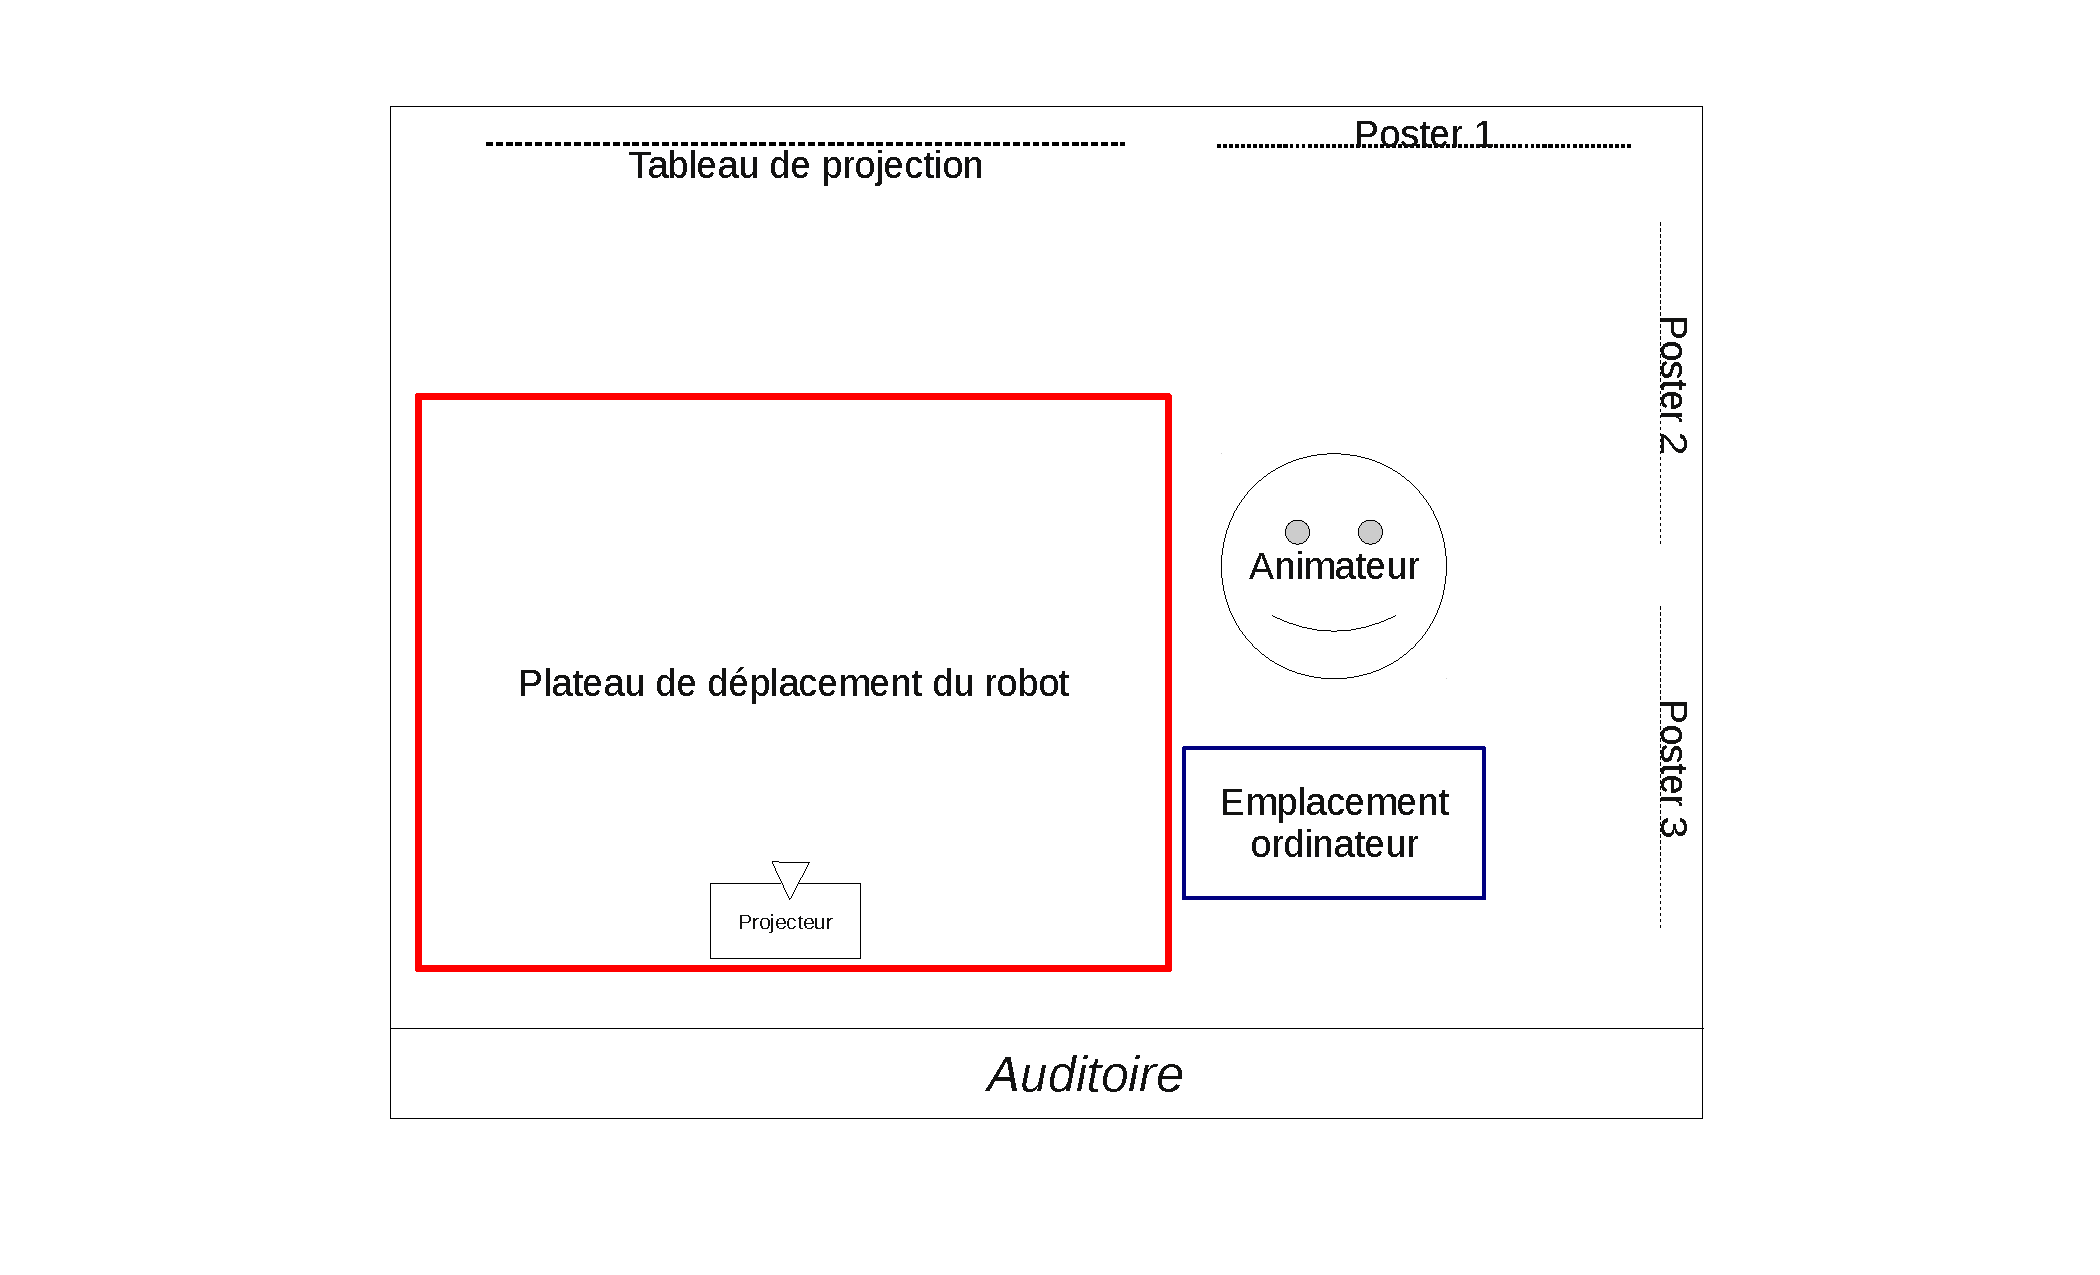
\includegraphics[width=14cm]{images/spatial}
\end{center}
\caption{Organisation spatiale de l'atelier (les proportions ne sont pas respectées).}
\label{fig:spatial-layout}
\end{figure}

D'une façon générale, chaque activité est dirigée par l'organisation temporelle suivante~: 
\begin{enumerate}
\item Un ou deux transparents (des extraits des posters) sont projetés
  et expliqués par l'animateur et se concluent par la formulation d'un problème.

\item L'auditoire est incité à donner son avis sur ce problème, à formuler des hypothèses.

\item Une expérimentation est conduite par l'animateur, éventuellement en collaboration avec l'auditoire. 

\item Un ou deux transparents (encore des extraits des posters)
  expliquent en termes plus généraux les concepts qui ont été utilisés
  pour la résolution du problème.

\end{enumerate}

\paragraph{Matériel} 
La description du robot, de sa construction aux outils utilisés pour
sa programmation, sera décrite dans une annexe technique de ce
document. Une part importante du matériel nécessaire concerne le
plateau. La figure~\ref{fig:plan} décrit ses différents composants. 

\begin{figure}
\begin{center}
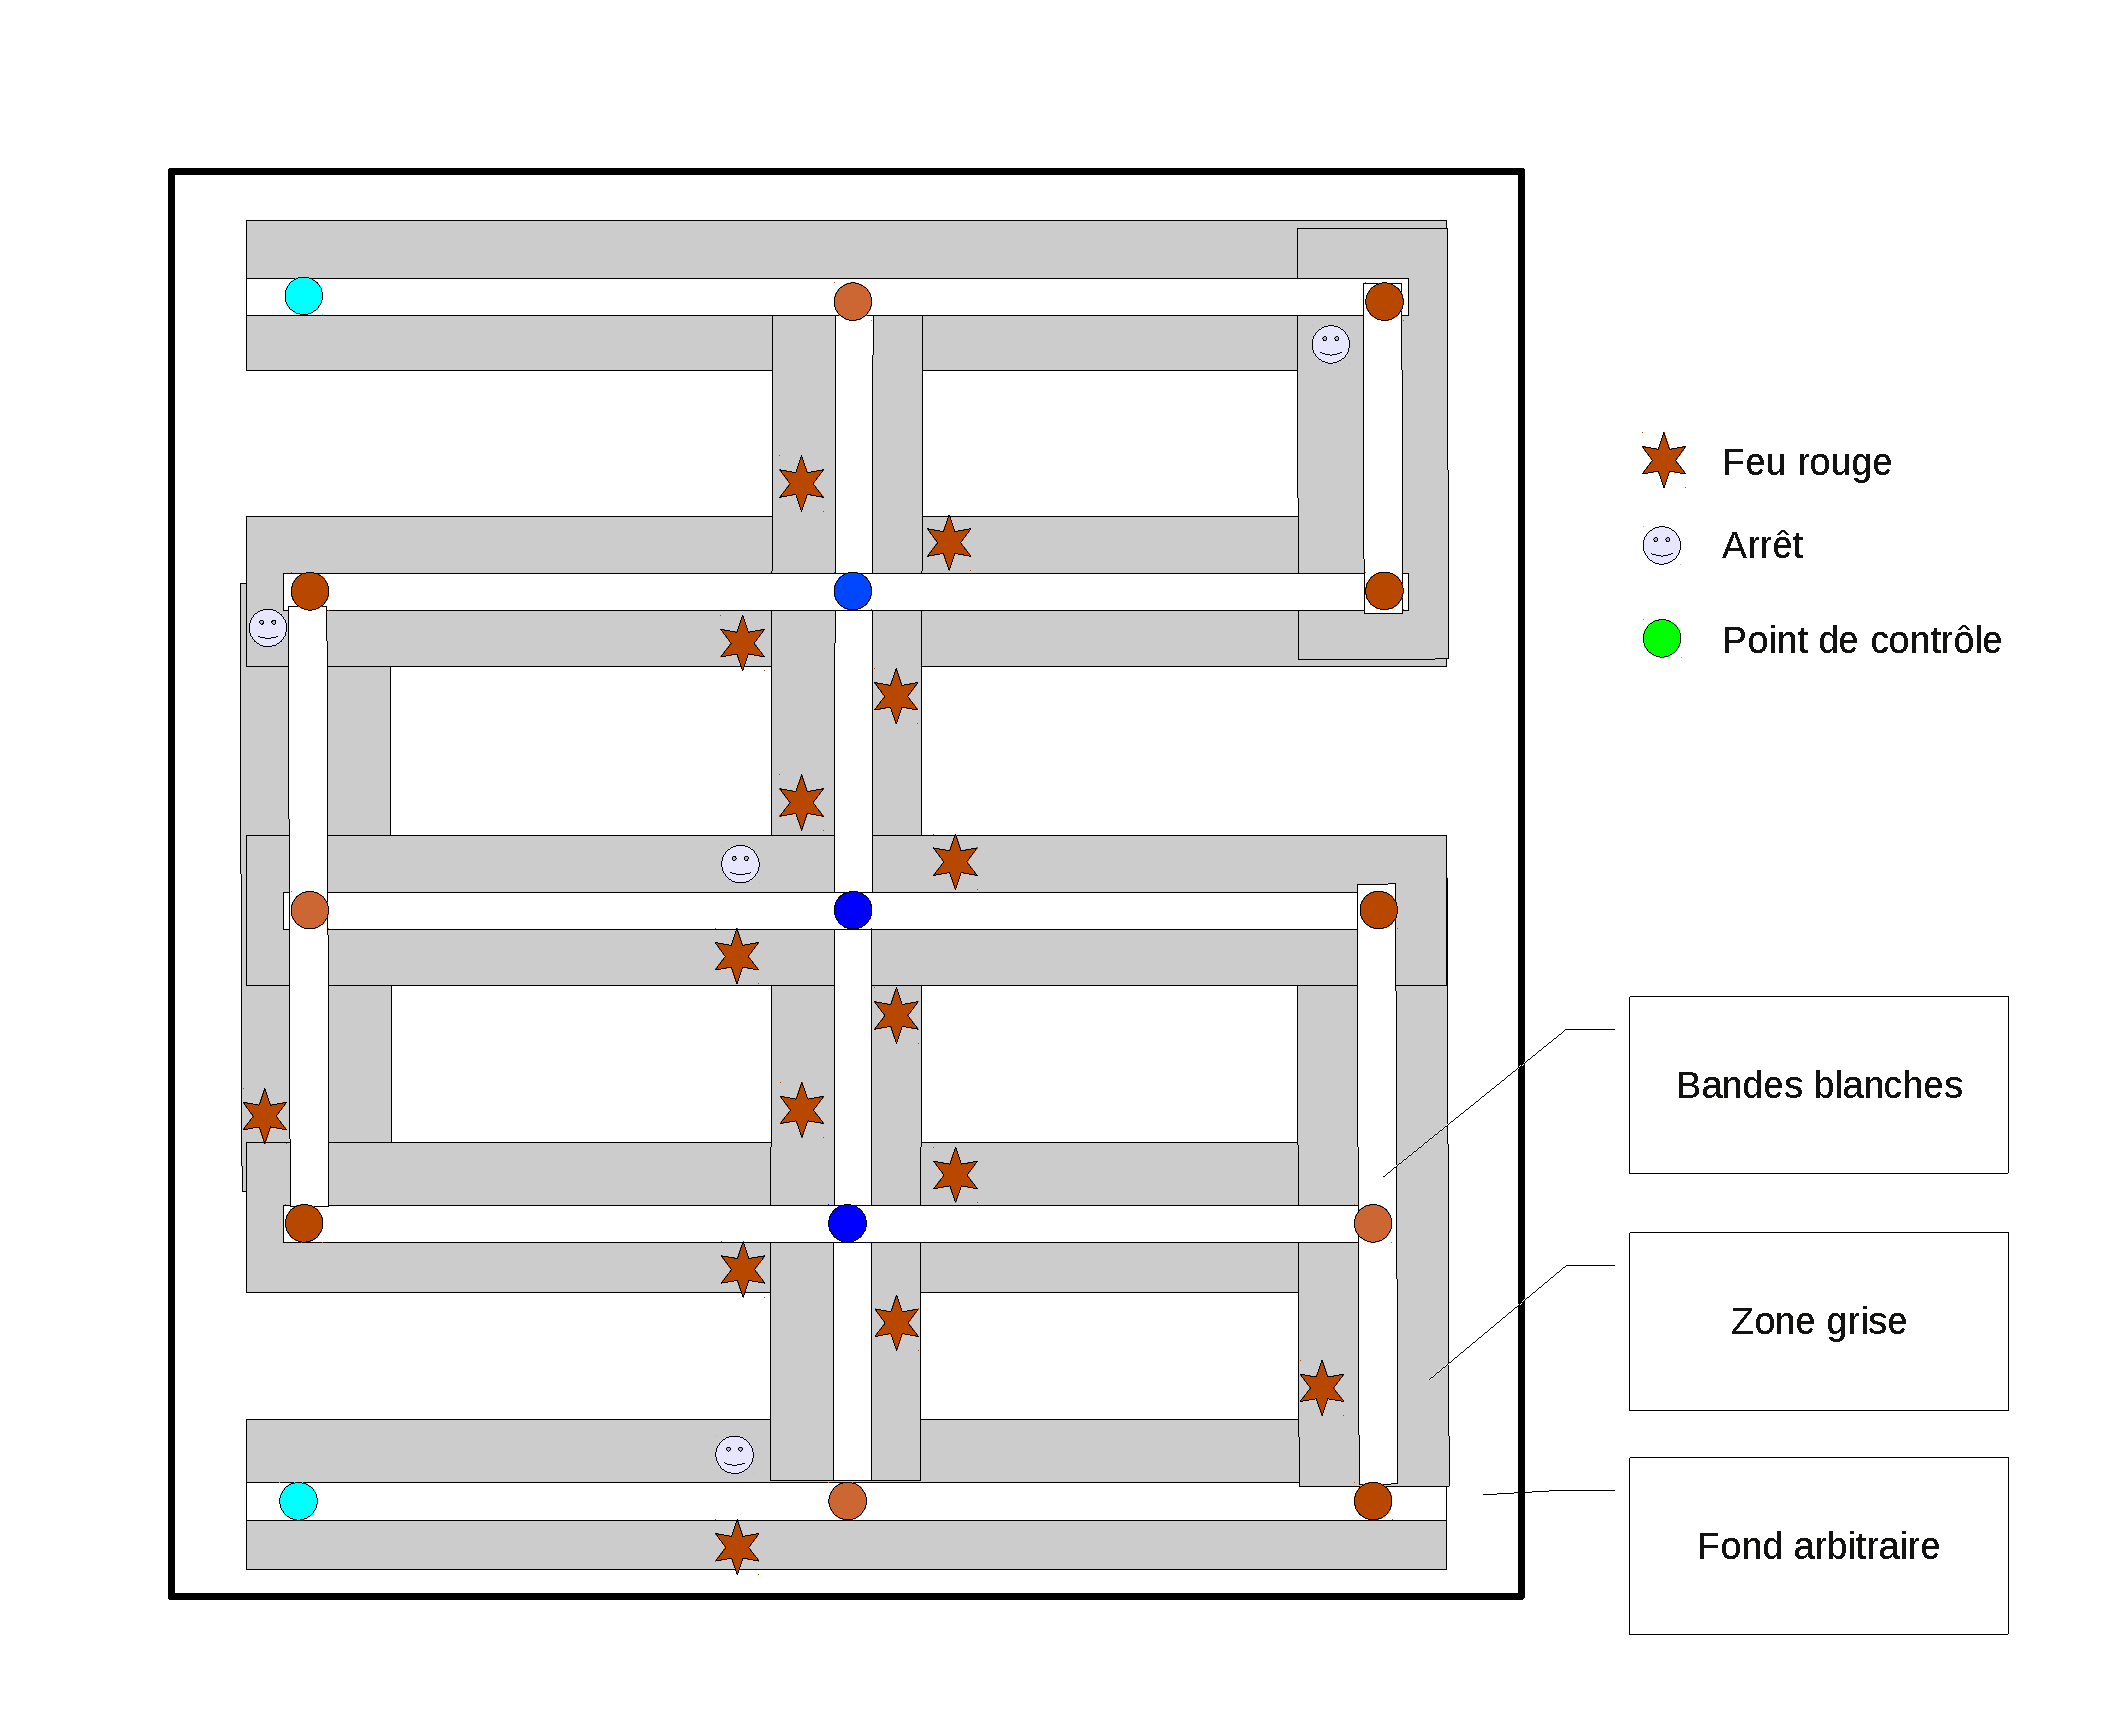
\includegraphics[width=14cm]{images/city}
\end{center}
\caption{Plan du quartier (les proportions ne sont pas respectées).}
\label{fig:plan}
\end{figure}

On y distingue~:
\begin{itemize}
\item des routes modélisées par une bande grise à l'intérieur de laquelle passe une bande blanche que
va suivre le robot; 

\item des points de contrôle servant à indiquer au robot qu'un choix ou une action particulière 
  est nécessaire ;

\item des feux rouges qui fixent des contraintes de pause au robot ;

\item des arrêts de bus qui modélisent les points où doit passer le robot.
\end{itemize}

Les dimensions des bandes et leur agencement sont contraintes par les
caractéristiques physiques du robot. Pour le reste, toute créativité
esthétique peut s'exprimer librement.

\subsection{Objectifs de dissémination de la culture scientifique}

Cet atelier vise à présenter l'outil informatique comme un outil pour
la résolution de problème, ce qui fait contraste avec sa fonctionnalité la
plus communément admise aujourd'hui d'outil de communication. Par ce
biais, on souhaite faire toucher du doigt la complexité inhérente à la
conception des systèmes informatiques et les méthodes scientifiques
qui permettent d'y parvenir, tant fondamentales qu'appliquées. 

Les problèmes abordés sont choisis pour leur accessibilité et leur
transversalité vis-à-vis des différents domaines de l'informatique. Du
point de vue de l'INRIA, on peut établir les associations suivantes
entre ces thèmes et les projets~:

\begin{itemize}
\item \textbf{Programmation}~: \textsc{Gallium}, \textsc{Contraintes}, \textsc{Moscova}, 
\textsc{ProVal}, $\pi r^2$, \textsc{Typical}, \textsc{Marelle}, \textsc{Abstraction}, 
\textsc{Formes}. 

\item \textbf{Automatique}~: \textsc{Aoste}, \textsc{Imara}.

\item \textbf{Algorithmique}~: \textsc{Algorithms}. 
\end{itemize}

\subsection{Objectifs pédagogiques}

Les objectifs pédagogiques de cet atelier diffèrent en fonction du niveau de l'auditoire. 

\subsubsection{Pré-élémentaire}

Pour éveiller les jeunes enfants à la technologie, il peut être plus
efficace de privilégier l'expérimentation tactile à travers une
interface la plus simple possible. Les algorithmes ne sont pas
inconnus des enfants~: dès la première année d'école pré-élémentaire,
le jeune élève suit par exemple des instructions de collage de
gommettes décritent en langage algorithmique. («~Deux gommettes rouges, un gommette bleue, 
et on recommence.~»)

La première activité est donc accessible aux jeunes enfants~: il
s'agit en effet de déterminer à l'avance une série de commandes parmi
trois actions ``avancer'', ``tourner à gauche'', ``tourner à droite''
puis de lancer ce programme sur le robot et d'observer le résultat.
Le dénombrement des actions à effectuer est un exercice accessible aux
enfants, à condition de rester dans un cadre manipulant de petites quantités. 

\subsubsection{Élémentaire}

Pour les élèves de l'école élémentaire, de nombreux domaines peuvent
être mis en relation avec cet atelier, parmi lesquels~: les
mathématiques, les sciences expérimentales, les langues, la lecture et
l'écriture. 

\paragraph{Mathématiques} 
Les algorithmes, en particulier de calculs arithmétiques, sont
au centre des apprentissages des mathématiques. La construction algorithmique ``tant que'' 
est utilisée par les enfants de l'école primaire. («~Pour diviser, j'essaie un numérateur 
plus grand tant que le reste n'est pas plus petit que le diviseur.~») 
Une partie de la solution à l'activité 2 utilise ce mécanisme. 

Par ailleurs, les calculs de plus court chemin sont accessibles à un
enfant d'école primaire. Même si la compréhension de la correction de
l'algorithme est hors de sa portée, il peut aussi constater
expérimentalement que, pour une instance donnée, parmi tous les
chemins possible l'algorithme choisi bien le plus court.

\paragraph{Sciences expérimentales}

On essaie de suivre la méthode scientifique pour toutes les activités:
formalisation/modélisation d'un problème, formulation d'une hypothèse
et vérification expérimentale. A priori, les élèves d'école primaire
sont initiés à ce processus. On tentera de faire comprendre la
distinction entre les données d'entrée de la solution théorique du
problème et les paramètres supplémentaires de sa solution pratique.
(«~Qu'arrive-t-il si on déplace le robot manuellement au milieu de
  l'exécution du programme?~»)

\paragraph{Langues, écriture et lecture}

Les compétences de lecture et d'écriture sont mise à l'épreuve à
partir de l'activité 2 car on y utilise un langage de programmation
exprimé dans un format textuel. L'utilisation d'un langage artificiel
(ici, le langage de programmation) peut offrir un nouveau regard sur
l'apprentissage de la grammaire, ou du vocabulaire, d'une nouvelle
langue. On tentera de formuler une distinction entre langage naturel
et langage artificiel. 


\subsubsection{Collège}

En plus des matières citées dans la section précédente, les enseignements du collège
les plus concernés par cet atelier sont la technologie et la physique. 

\paragraph{Mathématiques}

Le programme de mathématique du collège est une voie vers
l'apprentissage de l'abstraction, c'est-à-dire de l'utilisation de
concepts pour représenter le monde et ses problèmes. 

La notion d'algorithme dépendant des caractéristiques d'une entrée
abstraite est approfondie au collège (par exemple, à travers les
premiers calculs formels). Les programmes informatiques sont des
exemples de manipulation d'objets formels (en opposition aux objets
numériques purement quantitatifs). La référence à la valeur
inconnue d'une variable dans le programme de l'activité 2 et le
raisonnement sur les composantes du graphe de l'activité 3 doivent
être accessibles à un élève de collège.

D'un point de vue géométrique, la direction du robot peut être modélisée
par un vecteur, objet mathématique au programme du collège. Dans la première
activité, l'interprétation de la série de commandes peut être donnée comme une 
somme de vecteurs. 

Les raisonnements de minimisation de quantité, abordés par la 3ème activité, peuvent
être en partie compris par un bon élève de collège. 

\paragraph{Physique}

La relation entre la rotation des moteurs et la distance de déplacement du robot et la relation
entre les vitesses de rotation relatives des moteurs et la rotation du robot nécessitent des
raisonnements de cinétique, au programme du collège. On peut aussi expliquer comment fonctionne
le capteur de couleurs du robot ainsi que la signification du flux de valeurs produit par
ce capteur. 

\paragraph{Technologie}

Le programme de technologie mentionne explicitement la programmation
parmi les compétences informatiques à acquérir. 

Par ailleurs, on pourra donner quelques explications sur la chaîne qui
mène du fichier textuel contenant le programme enregistré sur
l'ordinateur portable à l'exécution de code machine par l'unité
centrale du robot. L'élève retrouvera alors le vocabulaire appris en
cours de technologie~: fichier, disque dur, réseau, processeur,
mémoire, \ldots

% {\small\url{http://media.education.gouv.fr/file/special_6/53/1/Programme_technologie_33531.pdf}}

\subsubsection{Lycée}

Au lycée, certes la formation scientifique se poursuit et
s'approfondit mais l'élève se pose aussi la question de son
orientation. Cet atelier peut être l'occasion de présenter ce que fait
un informaticien, chercheur ou non. La méthodologie générale de la
décomposition d'un problème en sous-problèmes peut aussi être apprécié
par les lycéens.

\paragraph{Mathématiques}

Le concept de ``fonction'' est au c{\oe}ur des mathématiques du
lycée. L'activité 2 présente un programme comme une fonction
produisant des sorties à partir d'entrées. L'activité 3 étudie la
fonction qui associe un coût à chaque itinéraire envisagé et calcule
le minimum de cette fonction.

Une introduction au langage logique est un des sujets des
mathématiques du lycée. L'analogie avec les langages informatiques
n'est pas qu'une coïncidence~: les règles des langages de
programmation sont très similaires à ceux de la logique.

Par ailleurs, la programmation d'algorithme de calculs sont des sujets
mentionnés explicitement dans les programmes du lycée.

\paragraph{Sciences de l'ingénieur}

Les méthodes de conception, de spécification, de réalisation et de
vérification d'un produit sont des thèmes de la matière «~Sciences de
  l'ingénieur~». La réalisation d'un programme informatique suit la
même discipline.

\paragraph{Sciences humaines}

Le thème du langage artificiel peut mener à des discussions autour du
langage et de la sémantique. On peut aussi s'interroger sur une société
où les robots prennent une place de plus en plus importante. Enfin, 
la définition du mot «~intelligence~» est une source inépuisable de débat.

\subsubsection{Enseignement supérieur}

En plus d'un approfondissement des notions présentées plus haut, deux
grands thèmes pourraient intéresser des étudiants en fonction de leur spécialité~: 

\begin{itemize}
\item Filières scientifiques~: la résolution algorithmique d'un problème (classique) de théorie
  des graphes et sa mise en {\oe}uvre robotique. 

\item Filières non scientifiques~: les aspects epistémologiques de
  l'informatique (ambivalence entre l'informatique comme science de la
  théorie abstraite du calcul automatisée et l'informatique comme une
  technologie dont les applications concrètes ont d'importantes
  répercutions sociétales).

\end{itemize}

\newpage
\section{Activité 0~: Introduction de l'atelier}

\subsection{Présentation}

Avant de commencer les activités à proprement parler, l'animateur de l'atelier
se présente, introduit le sujet «~Apprendre la programmation avec un robot~»,
décrit les différentes composantes de l'atelier ainsi que le problème
général à résoudre~: «~Programmer le robot pour qu'il passe par tous les arrêts
où l'attendent des enfants en un minimum de temps~». 

\subsection{Discours}

À préciser. 

\subsection{Interactions possibles} L'animateur peut demander à son auditoire si il
a une idée des problèmes qu'ils vont rencontrer pour résoudre le problème. 

\section{Activité 1~: Un robot qui se commande à l'aide d'un ordinateur}
\label{sec:act1}

\subsection{Présentation}

Cette activité vise à expliquer le processus de programmation qui
consiste à~:
\begin{enumerate}
\item décrire des commandes dans un langage que comprenne les
humains, 

\item traduire cette description (le programme) en du langage machine

\item lancer l'exécution de ces commandes par le robot. 

\end{enumerate}

Pour cela, on se dote d'un langage d'un langage de programmation
visuel très simple car composé uniquement de trois types de commande
(aller tout droit en faisant un tour de roue, tourner d'un quart de
tour vers la gauche ou vers la droite) symbolisées par trois dessins
distincts. Un programme est alors une séquence de ces commandes.

Le problème à résoudre est de déplacer le robot d'un point A à un
point B de la ville en écrivant un programme. 

Après avoir trouvé la solution avec le public, on explique le
fonctionnement de la chaîne de programmation à un niveau de détails
plus ou moins poussé (en fonction de l'audience).

\subsection{Discours}

À préciser. 

\subsection{Poster}

À préciser. 

\subsection{Interactions possibles}

C'est l'auditoire qui propose une première solution. (Si la solution
est incorrecte, l'animateur fournit la bonne.) On peut éventuellement
faire taper la solution à une personne du public\ldots

\newpage
\section{Activité 2~: Un robot qui fonctionne (presque) tout seul}
\label{sec:act2}

\subsection{Présentation}

La précédente activité nécessite beaucoup d'intervention humaine~: on
aimerait que notre robot soit plus malin pour que nous puissions nous
occuper de choses plus intéressantes!

Pour exprimer des programmes plus compliqués, on se propose d'utiliser
une description des commandes plus évoluées, proche mais différente du
langage parlé~: un langage de programmation. 

On explique ce qu'est un langage de programmation~: il a une grammaire très
précise (montrer des erreurs de syntaxe que l'ordinateur rejette) ainsi qu'une
sémantique non ambiguë. On montre le programme précédent écrit dans
ce langage, on le traduit et on l'exécute. 

Une des choses ``plus intelligentes'' que l'on peut exprimer est
la boucle ``repete''. Elle permet de répéter plusieurs fois la même
action. On réécrit le programme avec une boucle ``repete''. 

En fonction de l'auditoire, on introduit plus ou moins précisément les
variables (non modifiables), les boucles ``tant que'' et les
expressions conditionnelles (``si~\ldots~alors~\ldots~sinon~\ldots'').

On explique ensuite comment construire des blocs réutilisables appelés
``fonctions'' qui servent à résoudre des problèmes à partir de problèmes
déjà résolus. Dans le cas qui nous intéresse, on montre comment 
résoudre le problème du suivi d'un itinéraire à l'aide d'une fonction
qui fait passer le robot d'un point de contrôle à un autre du plan. 

\subsection{Discours}

À préciser. 

\subsection{Poster}

À préciser. 

\subsection{Interactions possibles}

On questionne l'auditoire en fonction de son niveau. 

\newpage
\section{Activité 3~: Un robot qui résout des problèmes (très précis)}
\label{sec:act3}

\subsection{Présentation}

Notre robot sait maintenant suivre un itinéraire mais c'est encore
trop de travail pour nous que de calculer le bon itinéraire pour aller
chercher tous les enfants en le moins de temps possible (sachant que
le robot doit s'arrêter à chaque feu rouge pendant une durée
prédéterminée et dépendante du feu considéré). 

On explique alors le problème en des termes plus abstraits (mais pas
trop) sur une carte projetée indiquant le temps d'attente de chaque
feu rouge. On essaie alors de résoudre le problème à la main. La
combinatoire du problème est décourageante! On réessaie sur un
problème plus petit avec succès. Une première méthode se dégage~: on
peut essayer tous les itinéraires possibles et choisir celui dont le
temps calculé est le plus petit. On programme alors la solution et
l'ordinateur la résout quelques secondes ! (Notons que l'on ralentit
volontairement la puissance de calcul pour que ce soit rapide mais que le
temps d'attente soit observable tout de même.) On remarque d'ailleurs
même si l'on change les paramètres du problème, cette méthode
fonctionne toujours! 

Si on compte le nombre d'itinéraires calculés, on s'aperçoit qu'il est
très grand et qu'heureusement que l'ordinateur calcule très vite.
Cependant, on remarque aussi que si la carte de la ville n'a qu'un
n{\oe}ud de plus, la résolution du problème est deux fois plus
lente. Cette solution ne peut donc fonctionner en pratique!

On explique alors un algorithme plus malin, l'algorithme de Dijsktra,
et on montre que la résolution du problème par cet algorithme est
instantanée, même sur la carte de la France. C'est certainement
l'algorithme utilisé dans nos GPS.

\subsection{Discours}

À préciser. 

\subsection{Poster}

À préciser. 

\subsection{Interactions possibles}

Encore une fois, en fonction du niveau de l'audience, on fait
participer le public à la recherche de la solution ainsi qu'à 
la programmation du robot. On demande aussi à une personne
de formuler une nouvelle instance du problème. 

\end{document}
